% This is text associated with the open textbook "Open Electromagnetics"
% See immediately below for author, date
% This work is licensed under the Creative Commons Attribution-ShareAlike 4.0 International License. (CC BY-SA 4.0) 
% To view a copy of the license, visit http://creativecommons.org/licenses/by-sa/4.0/

%ORB TITLE Types of Transmission Lines
%ORB AUTHOR 0        # S.W. Ellingson, Virginia Tech (ellingson@vt.edu)
%ORB DATE 20180802   # yyyymmdd
%ORB ABSTRACT TEM vs. higher-order lines, quick overview of coax vs. microstrip vs. optical fiber etc.

\label{m0144_Types_of_Transmission_Lines} % <-- Must match name of this file and module directory name.  Don't mess with this!

Two common types of transmission line are
coaxial line 
\index{transmission line!coaxial}
\index{coax|see{transmission line}}
(Figure~\ref{m0028_fCoax}) and
microstrip line
\index{microstrip} 
(Figure~\ref{m0028_fMicrostrip}). 
Both are examples of \emph{transverse electromagnetic} (TEM) 
transmission lines.
A TEM line employs a single electromagnetic wave ``mode'' 
\index{mode}
having electric and magnetic field vectors in directions perpendicular to the axis of the line, as shown in Figures~\ref{m0144_fCoaxFieldStructure} and \ref{m0144_fMicrostripFieldStructure}.
%
TEM transmission lines appear primarily in radio frequency applications.
%
\begin{figure}[b!]
\begin{center}
\pdftooltip{{  % note double braces
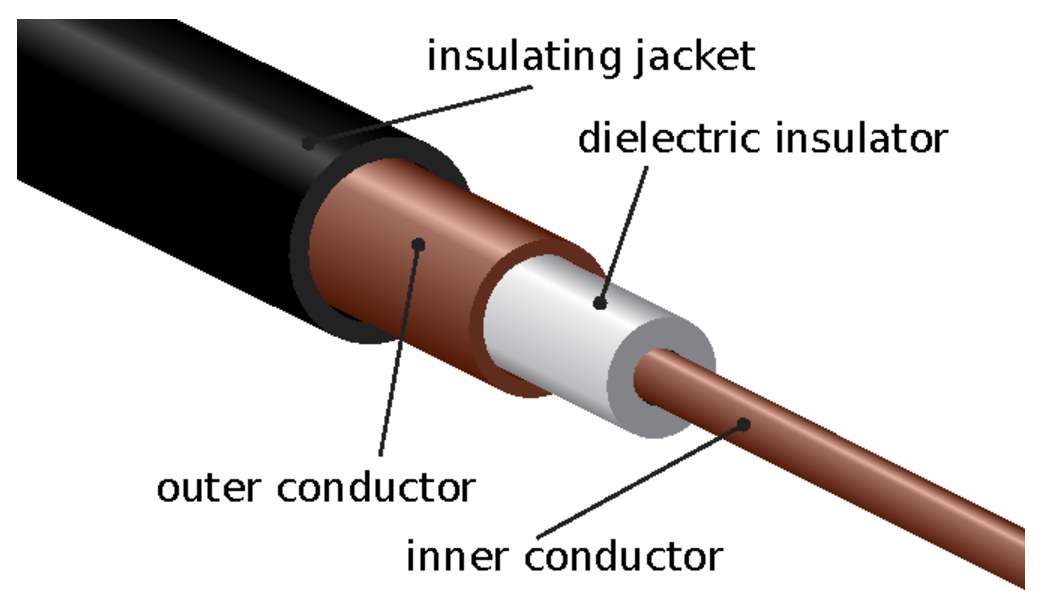
\includegraphics[width=2.5in]{modules/m0144_fCoaxial_cable_cutaway_170323se.eps}
% https://commons.wikimedia.org/wiki/File:Coaxial_cable_cutaway.svg
}}{The inner copper conductor wire is surrounded by a white dielectric insulator which is surrounded by an outer copper conductor layer which is surrounded by a black insulating jacket.}
\end{center} 
\centerline{\scriptsize 
\copyright~\hyperref[m0028_fCoax_Credit]{Tkgd2007} 
\href{https://creativecommons.org/licenses/by/3.0/}{CC BY 3.0} (modified)
} 
\caption{
\label{m0028_fCoax}
Structure of a coaxial transmission line. 
}
\end{figure}
%
\begin{figure}
\begin{center}
\pdftooltip{{  % note double braces
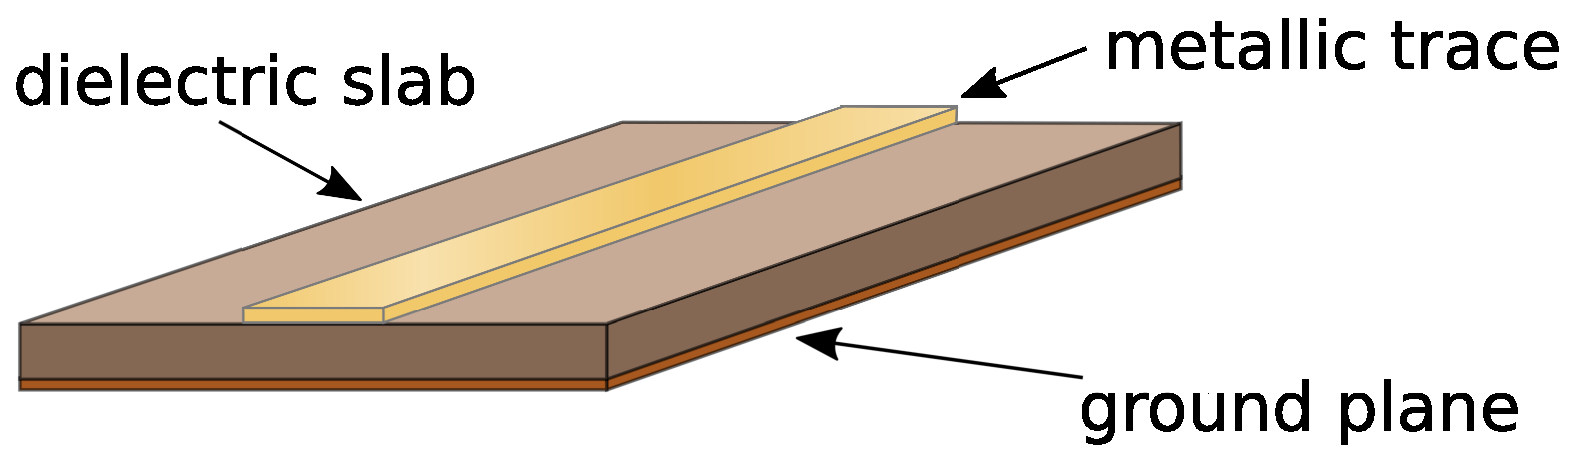
\includegraphics[width=2.5in]{modules/m0144_Microstrip_structure_170802se.eps}
% https://en.wikipedia.org/wiki/File:Microstrip_structure.svg
}}{A very thin, rectangular dielectric slab is set on the ground plane. Running longwise down the center of the dielectric slab is a thin layer of metallic trace.}
\end{center} 
\centerline{\scriptsize 
\copyright~\hyperref[m0028_fMicrostrip_Credit]{SpinningSpark} 
\href{https://creativecommons.org/licenses/by-sa/3.0/}{CC BY~SA 3.0} (modified)
} 
\caption{
\label{m0028_fMicrostrip}
Structure of a microstrip transmission line.
}
\end{figure}
%
\begin{figure}
\begin{center}
\pdftooltip{{  % note double braces
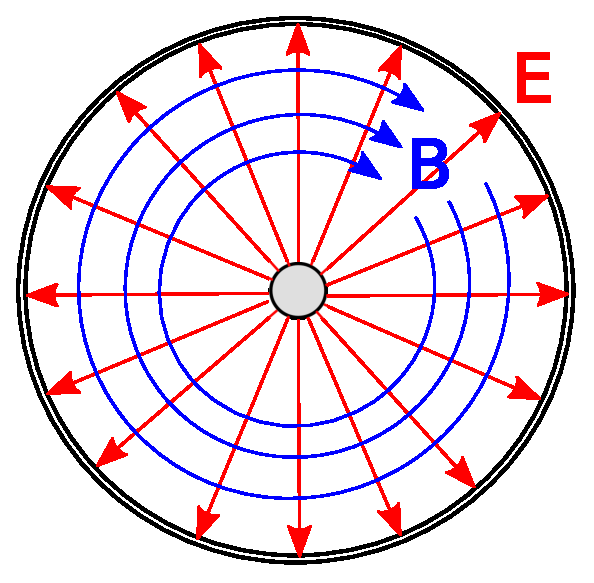
\includegraphics[width=1.5in]{modules/m0144_fCoaxFieldStructure.eps}
}}{A cross-sectional view of a coaxial transmission line. The inner conductor is represented by a gray-filled circle.  The electric field, "E", is represented by red arrows pointing outward from the inner conductor to the outer conductor which is represented by a larger concentric circle. The magnetic field, "B" is represented by concentric, circular blue arrows between the insulating jacket and the inner conductor. The arrows indicate a clockwise direction.}
\end{center} 
%\vspace{2.5in}
\caption{\label{m0144_fCoaxFieldStructure}Structure of the electric and magnetic fields within coaxial line.  In this case, the wave is propagating away from the viewer.}
\end{figure}
%
\begin{figure}
\begin{center}
\pdftooltip{{  % note double brace
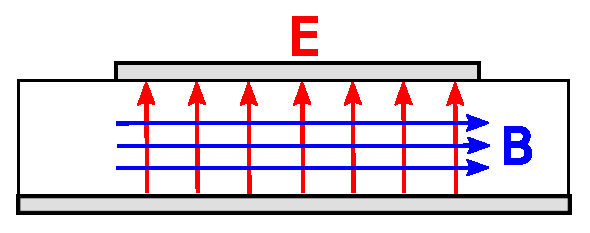
\includegraphics[width=2.0in]{modules/m0144_fMicrostripFieldStructure.eps}
}}{A cross-sectional view of a microstrip line. The electric field "E" is represented by a row of red parallel arrows pointing vertically from the ground plane to the metallic trace. The magnetic field "B" is represented by parallel blue arrows perpendicular to the electric field arrows, pointing to the right.}
\end{center} 
%\vspace{2.5in}
\caption{\label{m0144_fMicrostripFieldStructure}Structure of the electric and magnetic fields within microstrip line. (The fields \emph{outside} the line are possibly significant, complicated, and not shown.)  In this case, the wave is propagating away from the viewer.}
\end{figure}

%ORB HIGHLIGHT
\begin{mdframed}[backgroundcolor=yellow!20,nobreak=true] 
TEM transmission lines 
\index{transmission line!transverse electromagnetic (TEM)}
\index{TEM line|see{transmission line}}
such as coaxial lines and microstrip lines are designed to support a single electromagnetic wave that propagates along the length of the transmission line with electric and magnetic field vectors perpendicular to the direction of propagation.
\end{mdframed}

Not all transmission lines exhibit TEM field structure.
In non-TEM transmission lines, the electric and magnetic field vectors that are not necessarily perpendicular to the axis of the line, and the structure of the fields is complex relative to the field structure of TEM lines. 
An example of a transmission line that exhibits non-TEM field structure is the waveguide 
\index{waveguide}
(see example in Figure~\ref{m0028_fWaveGuide}).
Waveguides are most prevalent at radio frequencies, and tend to appear in applications where it is important to achieve very low loss or where power levels are very high.
Another example is common ``multimode'' optical fiber (Figure~\ref{m0028_fOpticalFiber}).
\index{optical fiber!multimode}
Optical fiber exhibits complex field structure because the wavelength of light is very small compared to the cross-section of the fiber, making the excitation and propagation of non-TEM waves difficult to avoid. (This issue is overcome in a different type of optical fiber, known as ``single mode'' fiber, 
\index{optical fiber!single mode}
which is much more difficult and expensive to manufacture.)  
%(Transmission lines for frequencies in the UV band and higher are not commonly encountered.)
%
\begin{figure}
\begin{center}
\pdftooltip{{  % note double braces
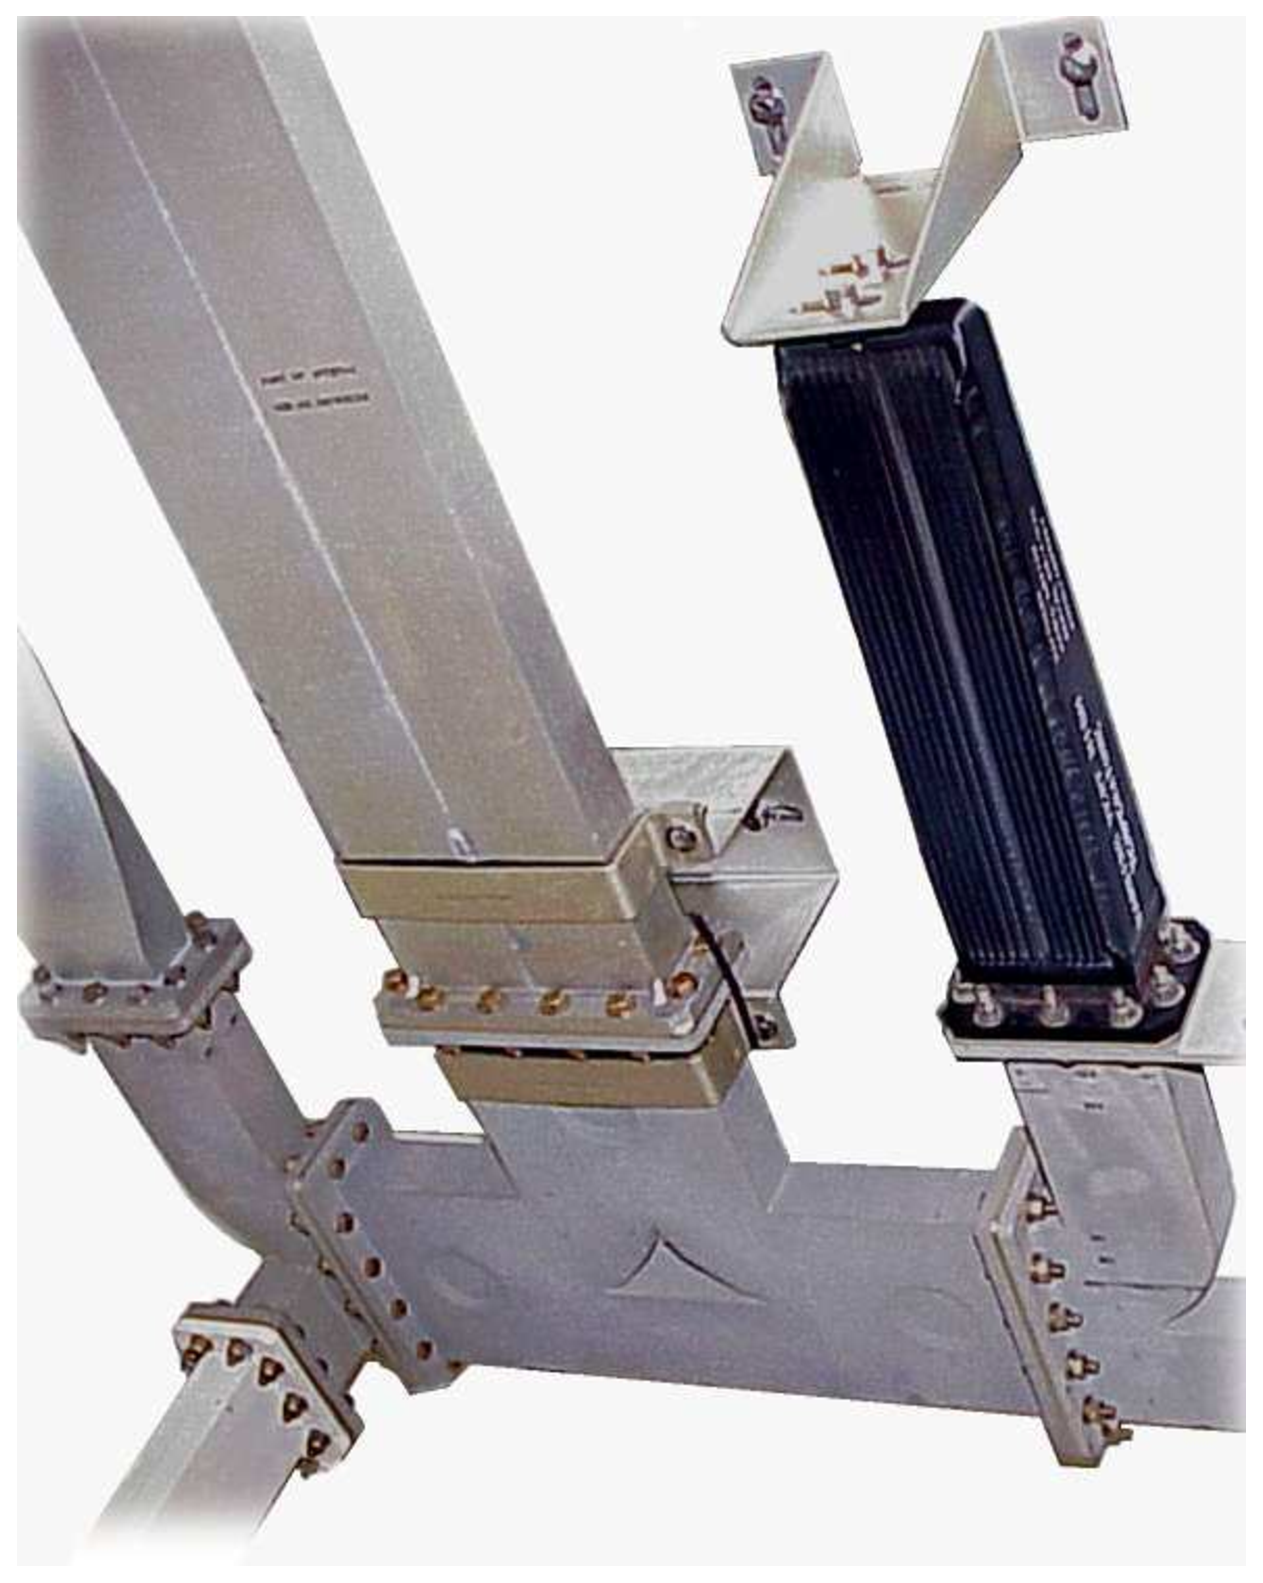
\includegraphics[width=2.5in]{modules/m0144_fDiplexer1.eps}
% https://en.wikipedia.org/wiki/File:Diplexer1.jpg
}}{Photo of waveguide highlighting multiple branching connections running in parallel.}
\end{center} 
\centerline{\scriptsize 
\copyright~\hyperref[m0028_fWaveGuide_Credit]{Averse} 
\href{https://creativecommons.org/licenses/by-sa/2.0/de/deed.en}{CC BY~SA 2.0 Germany} 
} 
\caption{
\label{m0028_fWaveGuide}
A network of radio frequency waveguides in an air traffic control radar.
}
\end{figure}
%
\begin{figure}
\begin{center}
\pdftooltip{{  % note double braces
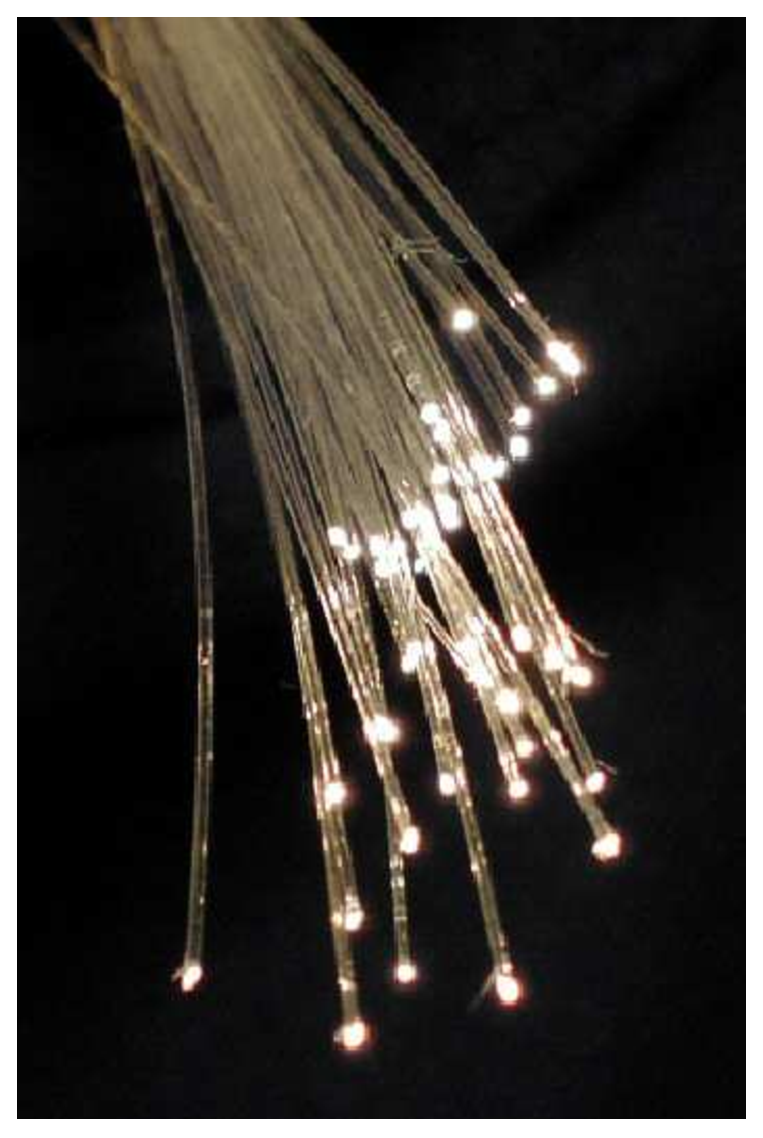
\includegraphics[width=1.5in]{modules/m0144_fFibreoptic.eps}
% https://en.wikipedia.org/wiki/File:Fibreoptic.jpg
}}{A bundle of clear, thin strands of fiber in a dark background. The tips of the fibers are glowing with white light.}
\end{center} 
\centerline{\scriptsize 
\copyright~\hyperref[m0028_fOpticalFiber_Credit]{BigRiz} 
\href{https://creativecommons.org/licenses/by-sa/3.0/deed.en}{CC BY~SA 3.0 Unported} 
} 
\caption{
\label{m0028_fOpticalFiber}
Strands of optical fiber.
}
\end{figure}

%ORB HIGHLIGHT
\begin{mdframed}[backgroundcolor=yellow!20,nobreak=true] 
Higher-order transmission lines, including radio-frequency waveguides and multimode optical fiber, are designed to guide waves that have relatively complex structure.
\end{mdframed}

%%%%%%%%%%%%%%%%%%%%%%%%%%%%%%%%%

{\bf Additional Reading:}
\begin{itemize}
\item ``\href{https://en.wikipedia.org/wiki/Coaxial_cable}{Coaxial cable}'' on Wikipedia.
\item ``\href{https://en.wikipedia.org/wiki/Microstrip}{Microstrip}'' on Wikipedia.
\item ``\href{https://en.wikipedia.org/wiki/Waveguide_(electromagnetism)}{Waveguide (electromagnetism)}'' on Wikipedia.
\item ``\href{https://en.wikipedia.org/wiki/Optical_fiber}{Optical fiber}'' on Wikipedia.
\end{itemize}

       

